\documentclass[aspectratio=169,10pt]{beamer}
\usetheme{Madrid}
\usecolortheme{whale}

\usepackage[utf8]{inputenc}
\usepackage[T5]{fontenc}
\usepackage[vietnamese]{babel}
\usepackage{booktabs}
\usepackage{graphicx}
\usepackage{amsmath}

\title[Đề tài 13 -- Nhóm 7]{BÀI TẬP LỚN NHẬP MÔN HỌC MÁY (FIT4013)\\Đề tài 13: Dự đoán nhân viên có khả năng nghỉ việc}
\subtitle{Nhóm đề tài: Dữ liệu dạng bảng (Tabular Data)}
\author[Nhóm 7 -- FIT4013]{%
    \textbf{Giảng viên hướng dẫn:} ThS. Lê Thị Thùy Trang\\[0.2cm]
    \textbf{Nhóm 7:} Nguyễn Văn An (1871020003) $\cdot$ Nguyễn Việt Anh (1871020047)\\
    Đào Thị Tươi (1871020639) $\cdot$ Lê Đình Huy (1871020307)%
}
\date{Tháng 11/2026}

\begin{document}

% Slide 1
\begin{frame}
    \titlepage
\end{frame}

% Slide 2
\begin{frame}{1. Đặt vấn đề và Khám phá dữ liệu (EDA)}
    \begin{columns}
        \begin{column}{0.48\textwidth}
            \textbf{Bối cảnh \& Mục tiêu:}
            \begin{itemize}
                \item Dự đoán sớm nhân viên có nguy cơ tự nguyện nghỉ việc (\texttt{Attrition = Yes}) để bộ phận HR kịp thời giữ chân.
                \item Bộ dữ liệu: \textbf{IBM HR Analytics} ($1{,}470$ mẫu $\times$ $35$ cột).
                \item Không có dữ liệu khuyết ($0$ missing), không có dòng trùng lặp.
                \item Phát hiện 4 cột không mang thông tin dự đoán: \texttt{EmployeeNumber} (ID), \texttt{EmployeeCount}, \texttt{Over18}, \texttt{StandardHours} (hằng số).
            \end{itemize}
        \end{column}
        \begin{column}{0.50\textwidth}
            \centering
            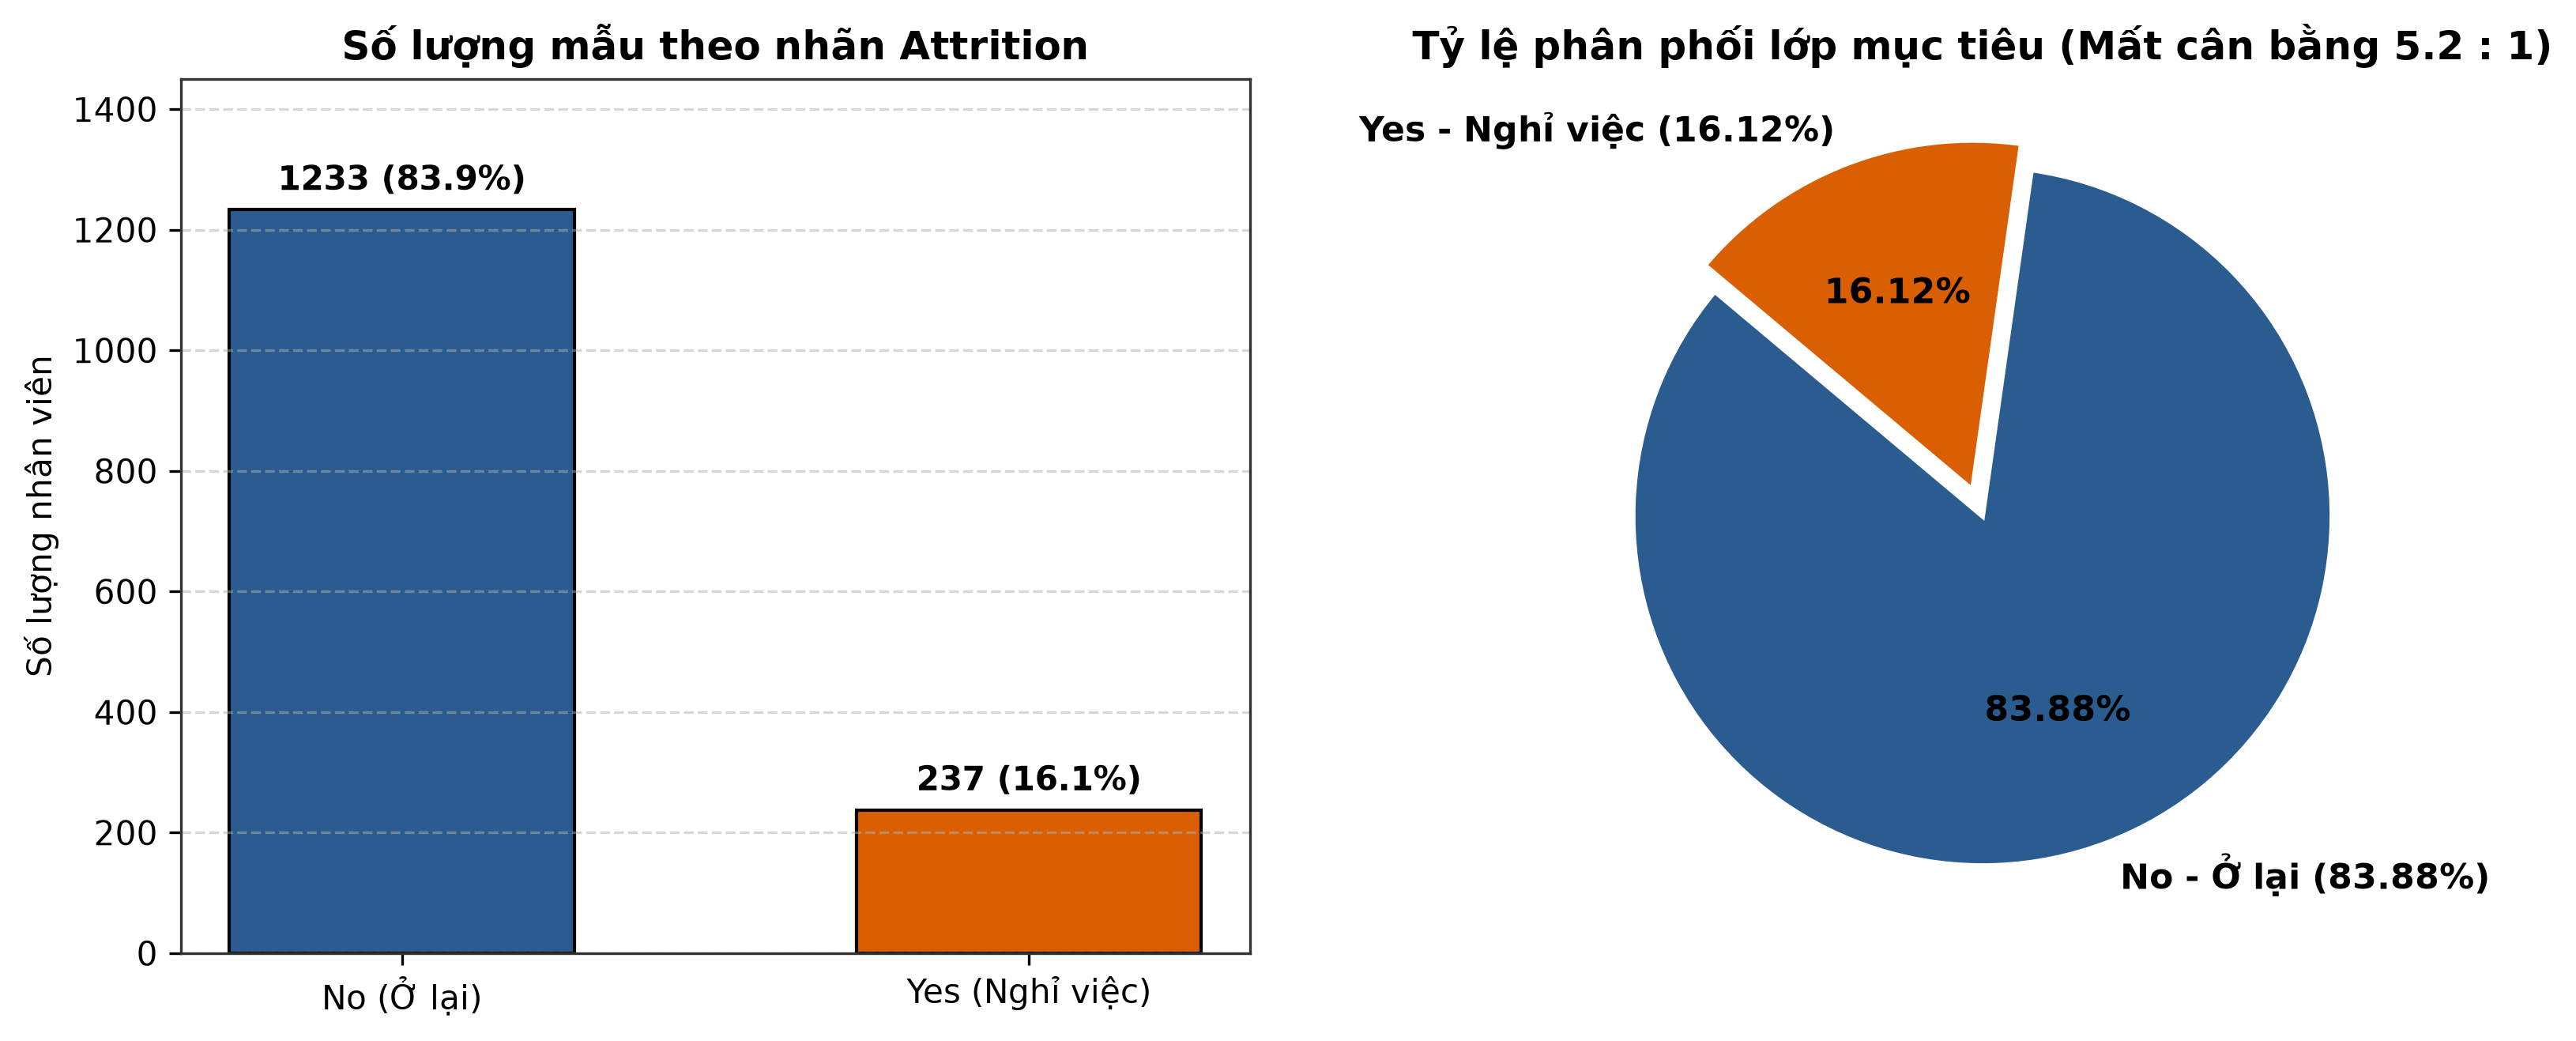
\includegraphics[width=\textwidth]{figures/fig1_target_distribution.png}
            \footnotesize \textbf{Mất cân bằng lớp ($5.2:1$):} Chỉ $16.12\%$ lớp \texttt{Yes} $\rightarrow$ Ưu tiên \textbf{F1-score, Recall, ROC-AUC} thay vì chỉ dùng Accuracy.
        \end{column}
    \end{columns}
\end{frame}

% Slide 3
\begin{frame}{2. Các phát hiện quan trọng từ EDA}
    \begin{columns}
        \begin{column}{0.50\textwidth}
            \centering
            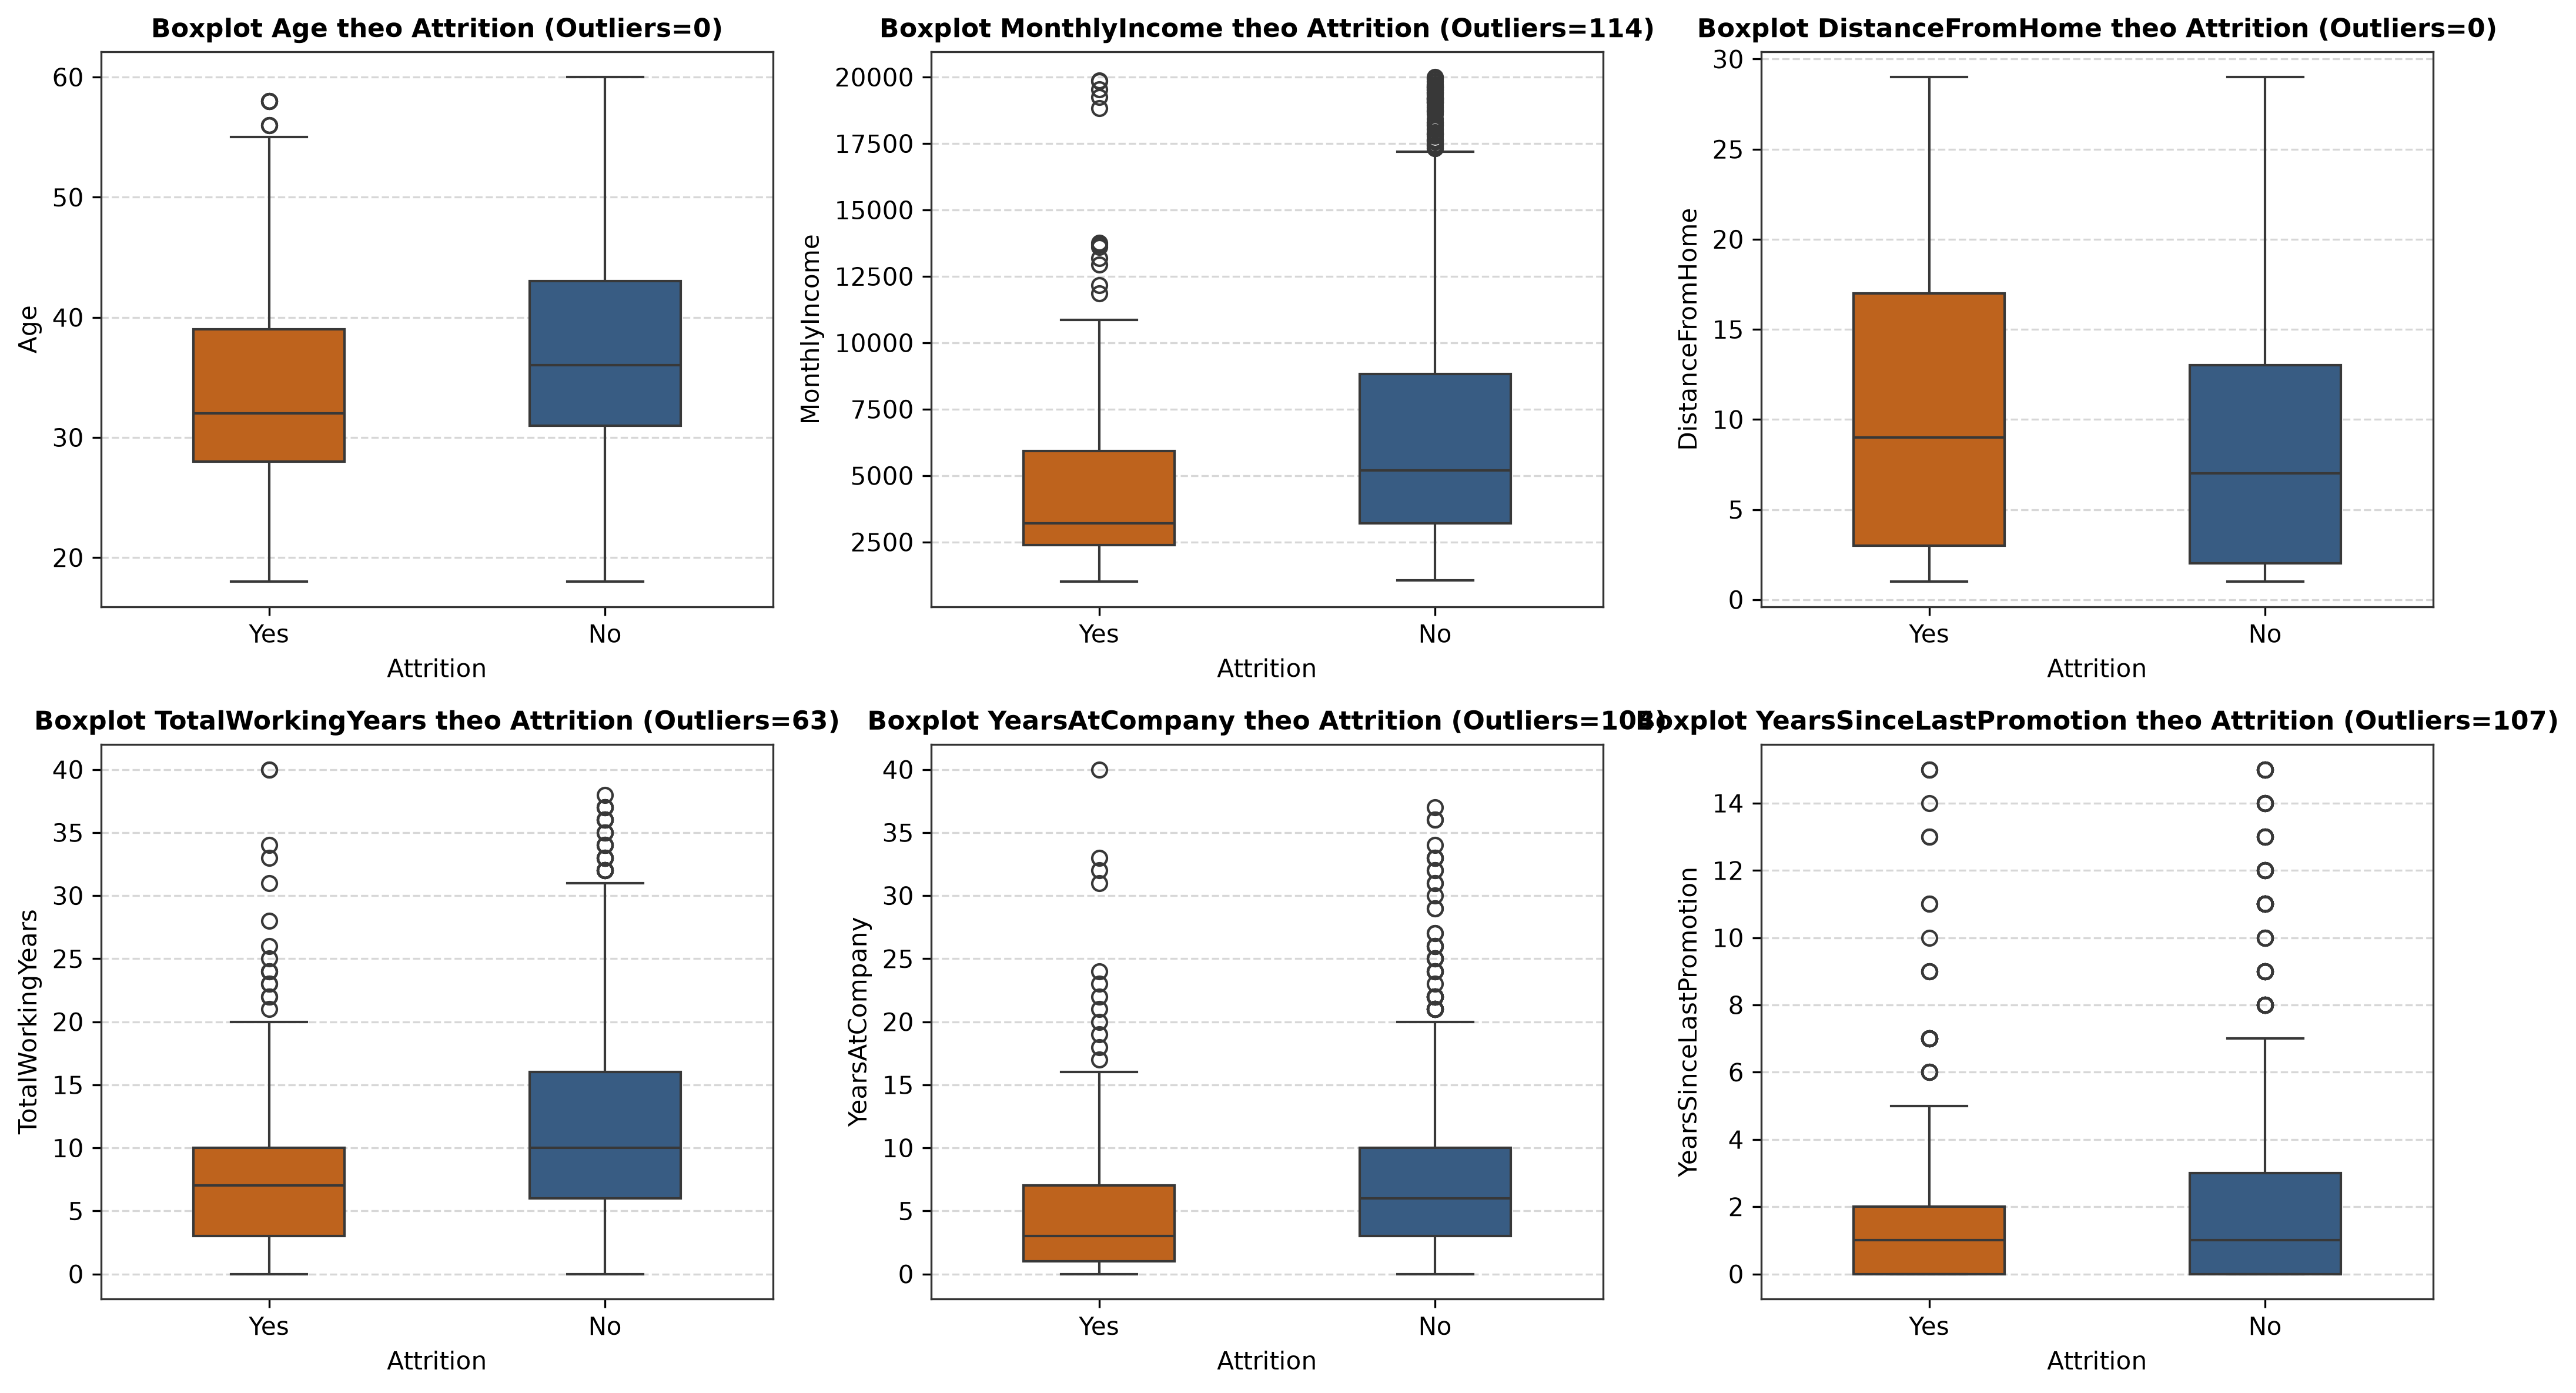
\includegraphics[width=\textwidth]{figures/fig2_numeric_distributions.png}
            \footnotesize Biến \texttt{MonthlyIncome}, \texttt{YearsAtCompany}, \texttt{YearsSinceLastPromotion} lệch phải mạnh (Skew $> 1.3$) và có $7\% - 8\%$ ngoại lệ IQR.
        \end{column}
        \begin{column}{0.50\textwidth}
            \centering
            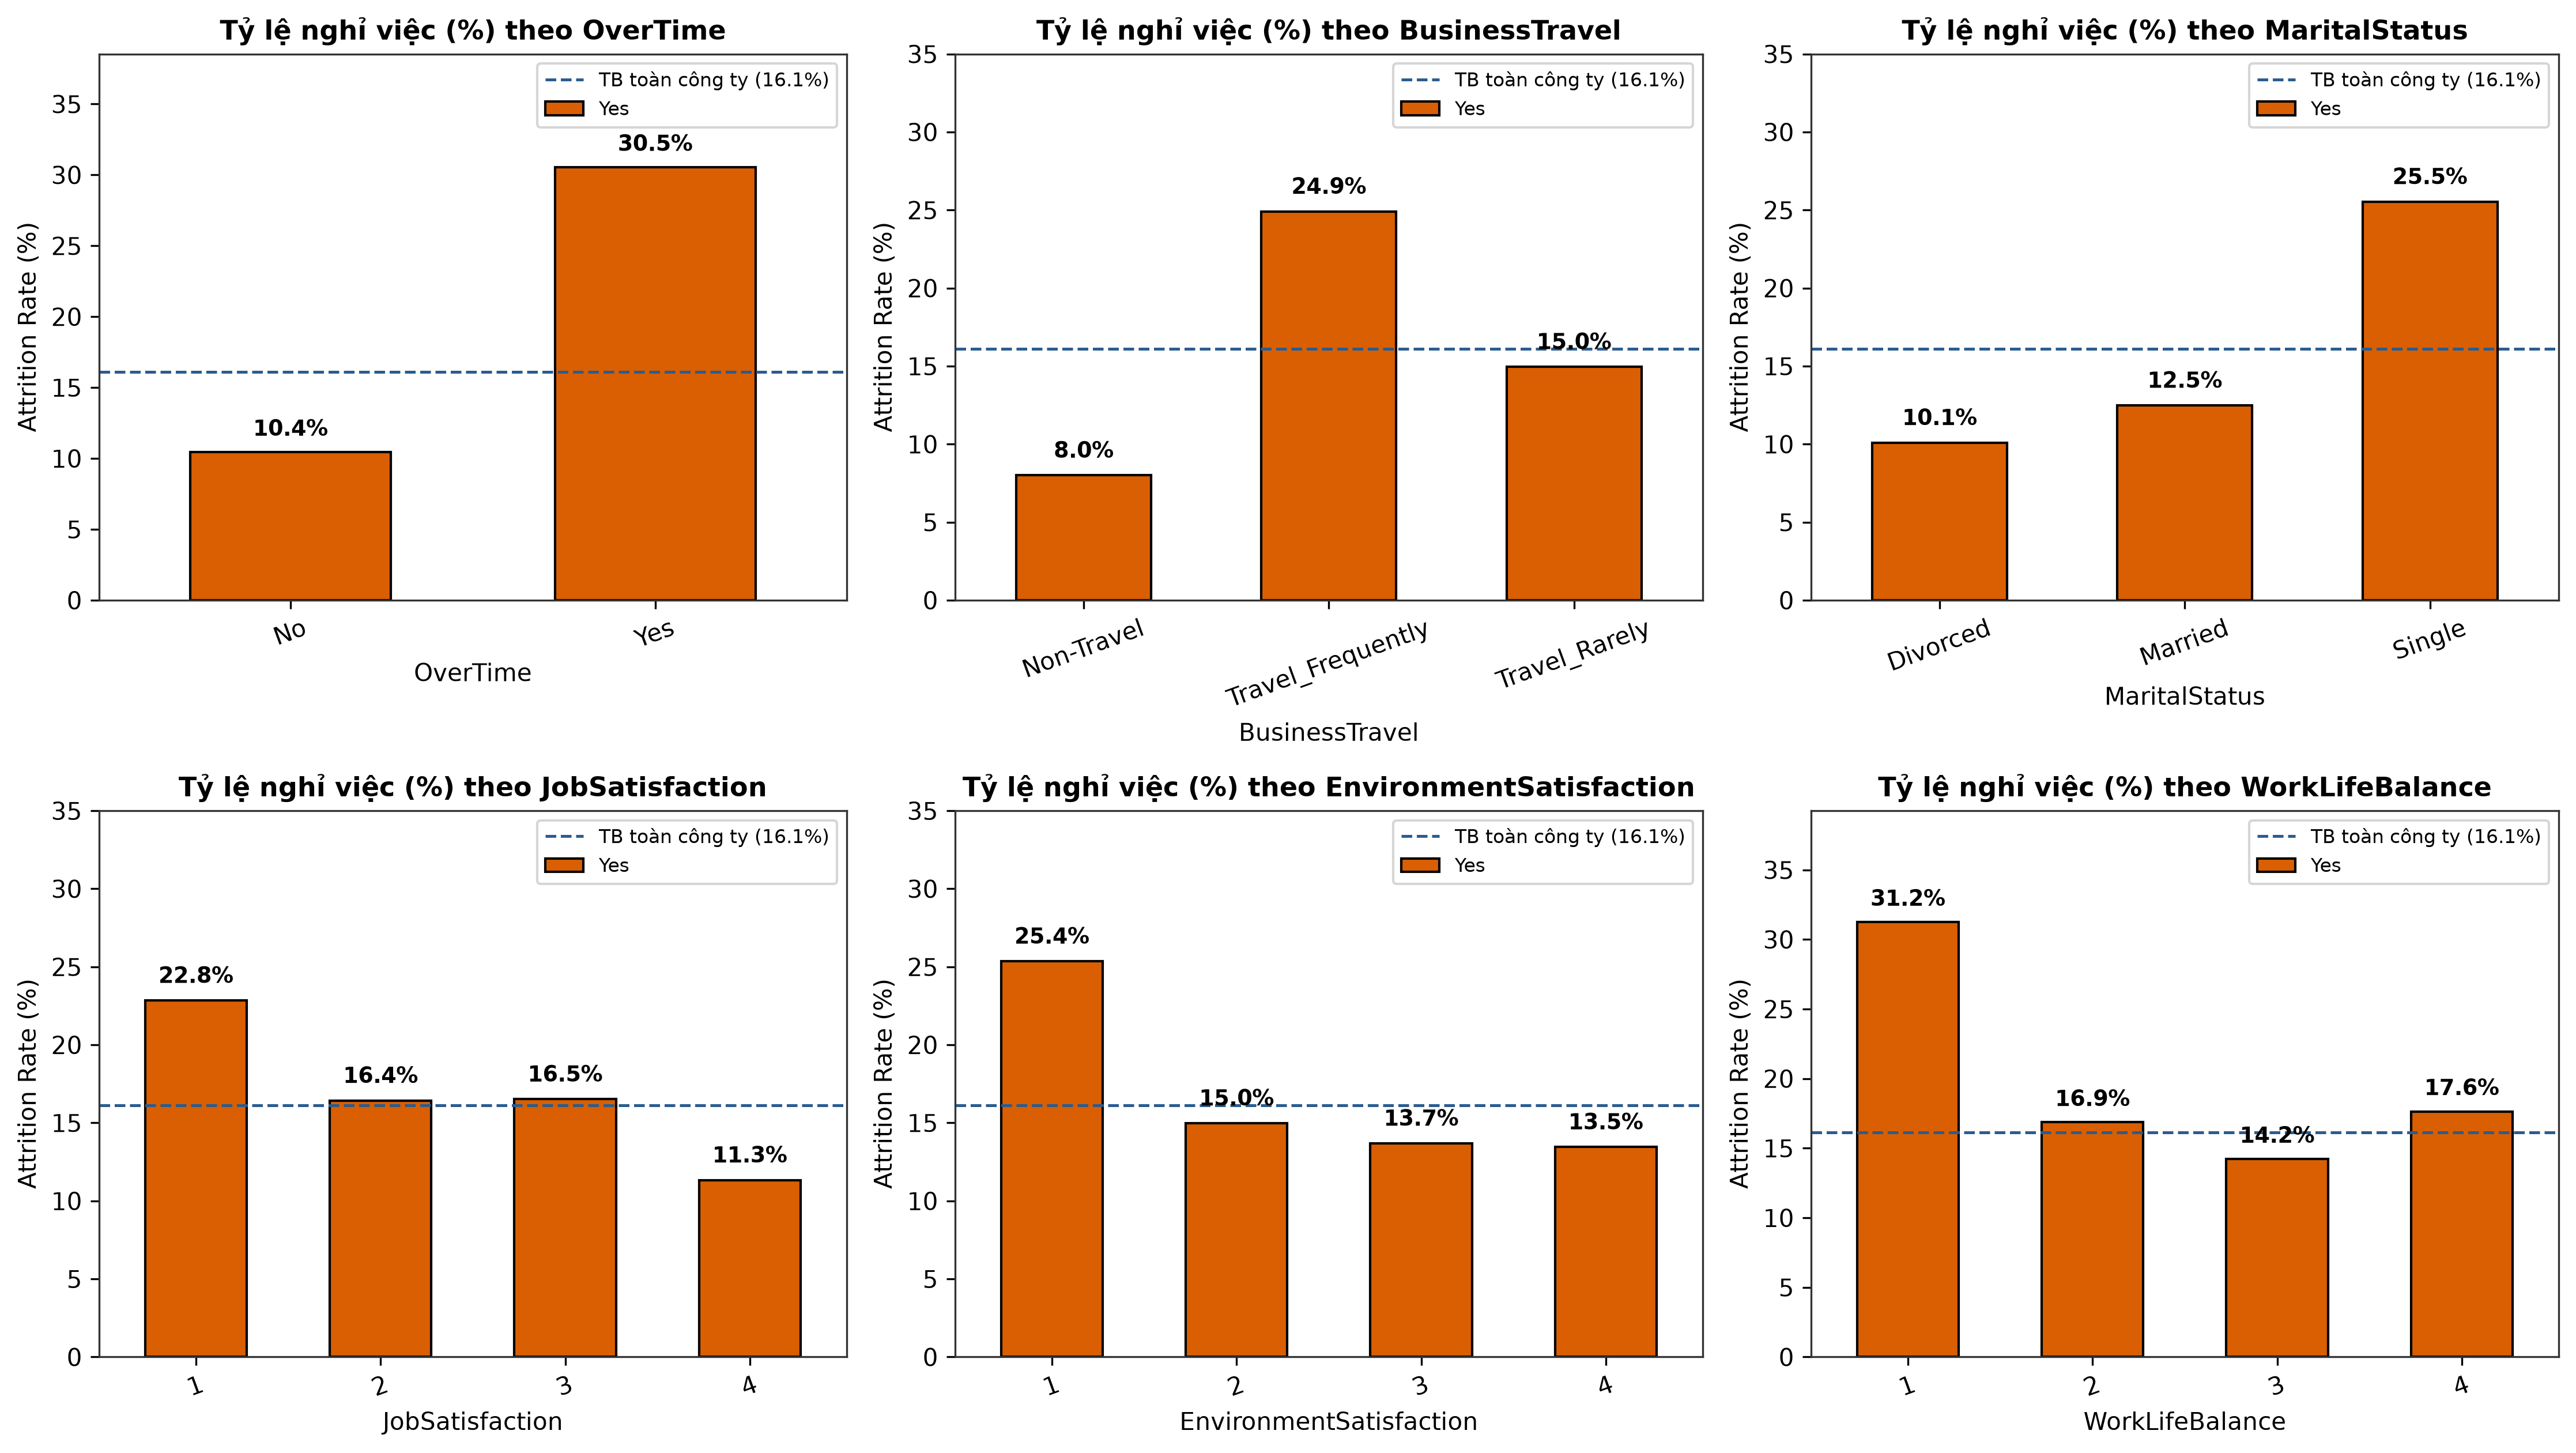
\includegraphics[width=\textwidth]{figures/fig3_categorical_attrition.png}
            \footnotesize Nhóm \texttt{OverTime = Yes} có tỷ lệ nghỉ việc \textbf{30.5\%} (gấp 3 lần nhóm No); nhóm \texttt{Travel\_Frequently} là \textbf{24.9\%}.
        \end{column}
    \end{columns}
\end{frame}

% Slide 4
\begin{frame}{3. Thiết kế 2 Luồng Tiền xử lý \& Kỹ thuật Đặc trưng}
    \begin{columns}
        \begin{column}{0.46\textwidth}
            \begin{block}{Luồng A: Pipeline Cơ bản (44 chiều)}
                \begin{itemize}
                    \item Bỏ 4 cột ID/hằng số.
                    \item \texttt{OneHotEncoder(drop='first')} cho 7 biến phân loại.
                    \item \texttt{StandardScaler} cho 23 biến số.
                \end{itemize}
            \end{block}
            \begin{alertblock}{Luồng B: Pipeline Cải tiến (46 chiều)}
                \begin{itemize}
                    \item \textbf{Tạo 7 đặc trưng HR mới:} \texttt{OverallSatisfaction}, \texttt{CompanyTenureRatio}, \texttt{IncomePerWorkingYear}, \texttt{OverTime\_FrequentTravel}, \texttt{YoungSingleLowIncome}...
                    \item Biến đổi $\log(1+x)$ + \texttt{RobustScaler} chống ngoại lệ.
                    \item Bỏ \texttt{JobLevel} ($r=0.95$ với lương) và 3 cột Rate nhiễu + Chọn lọc \texttt{SelectKBest(f\_classif)}.
                \end{itemize}
            \end{alertblock}
        \end{column}
        \begin{column}{0.52\textwidth}
            \centering
            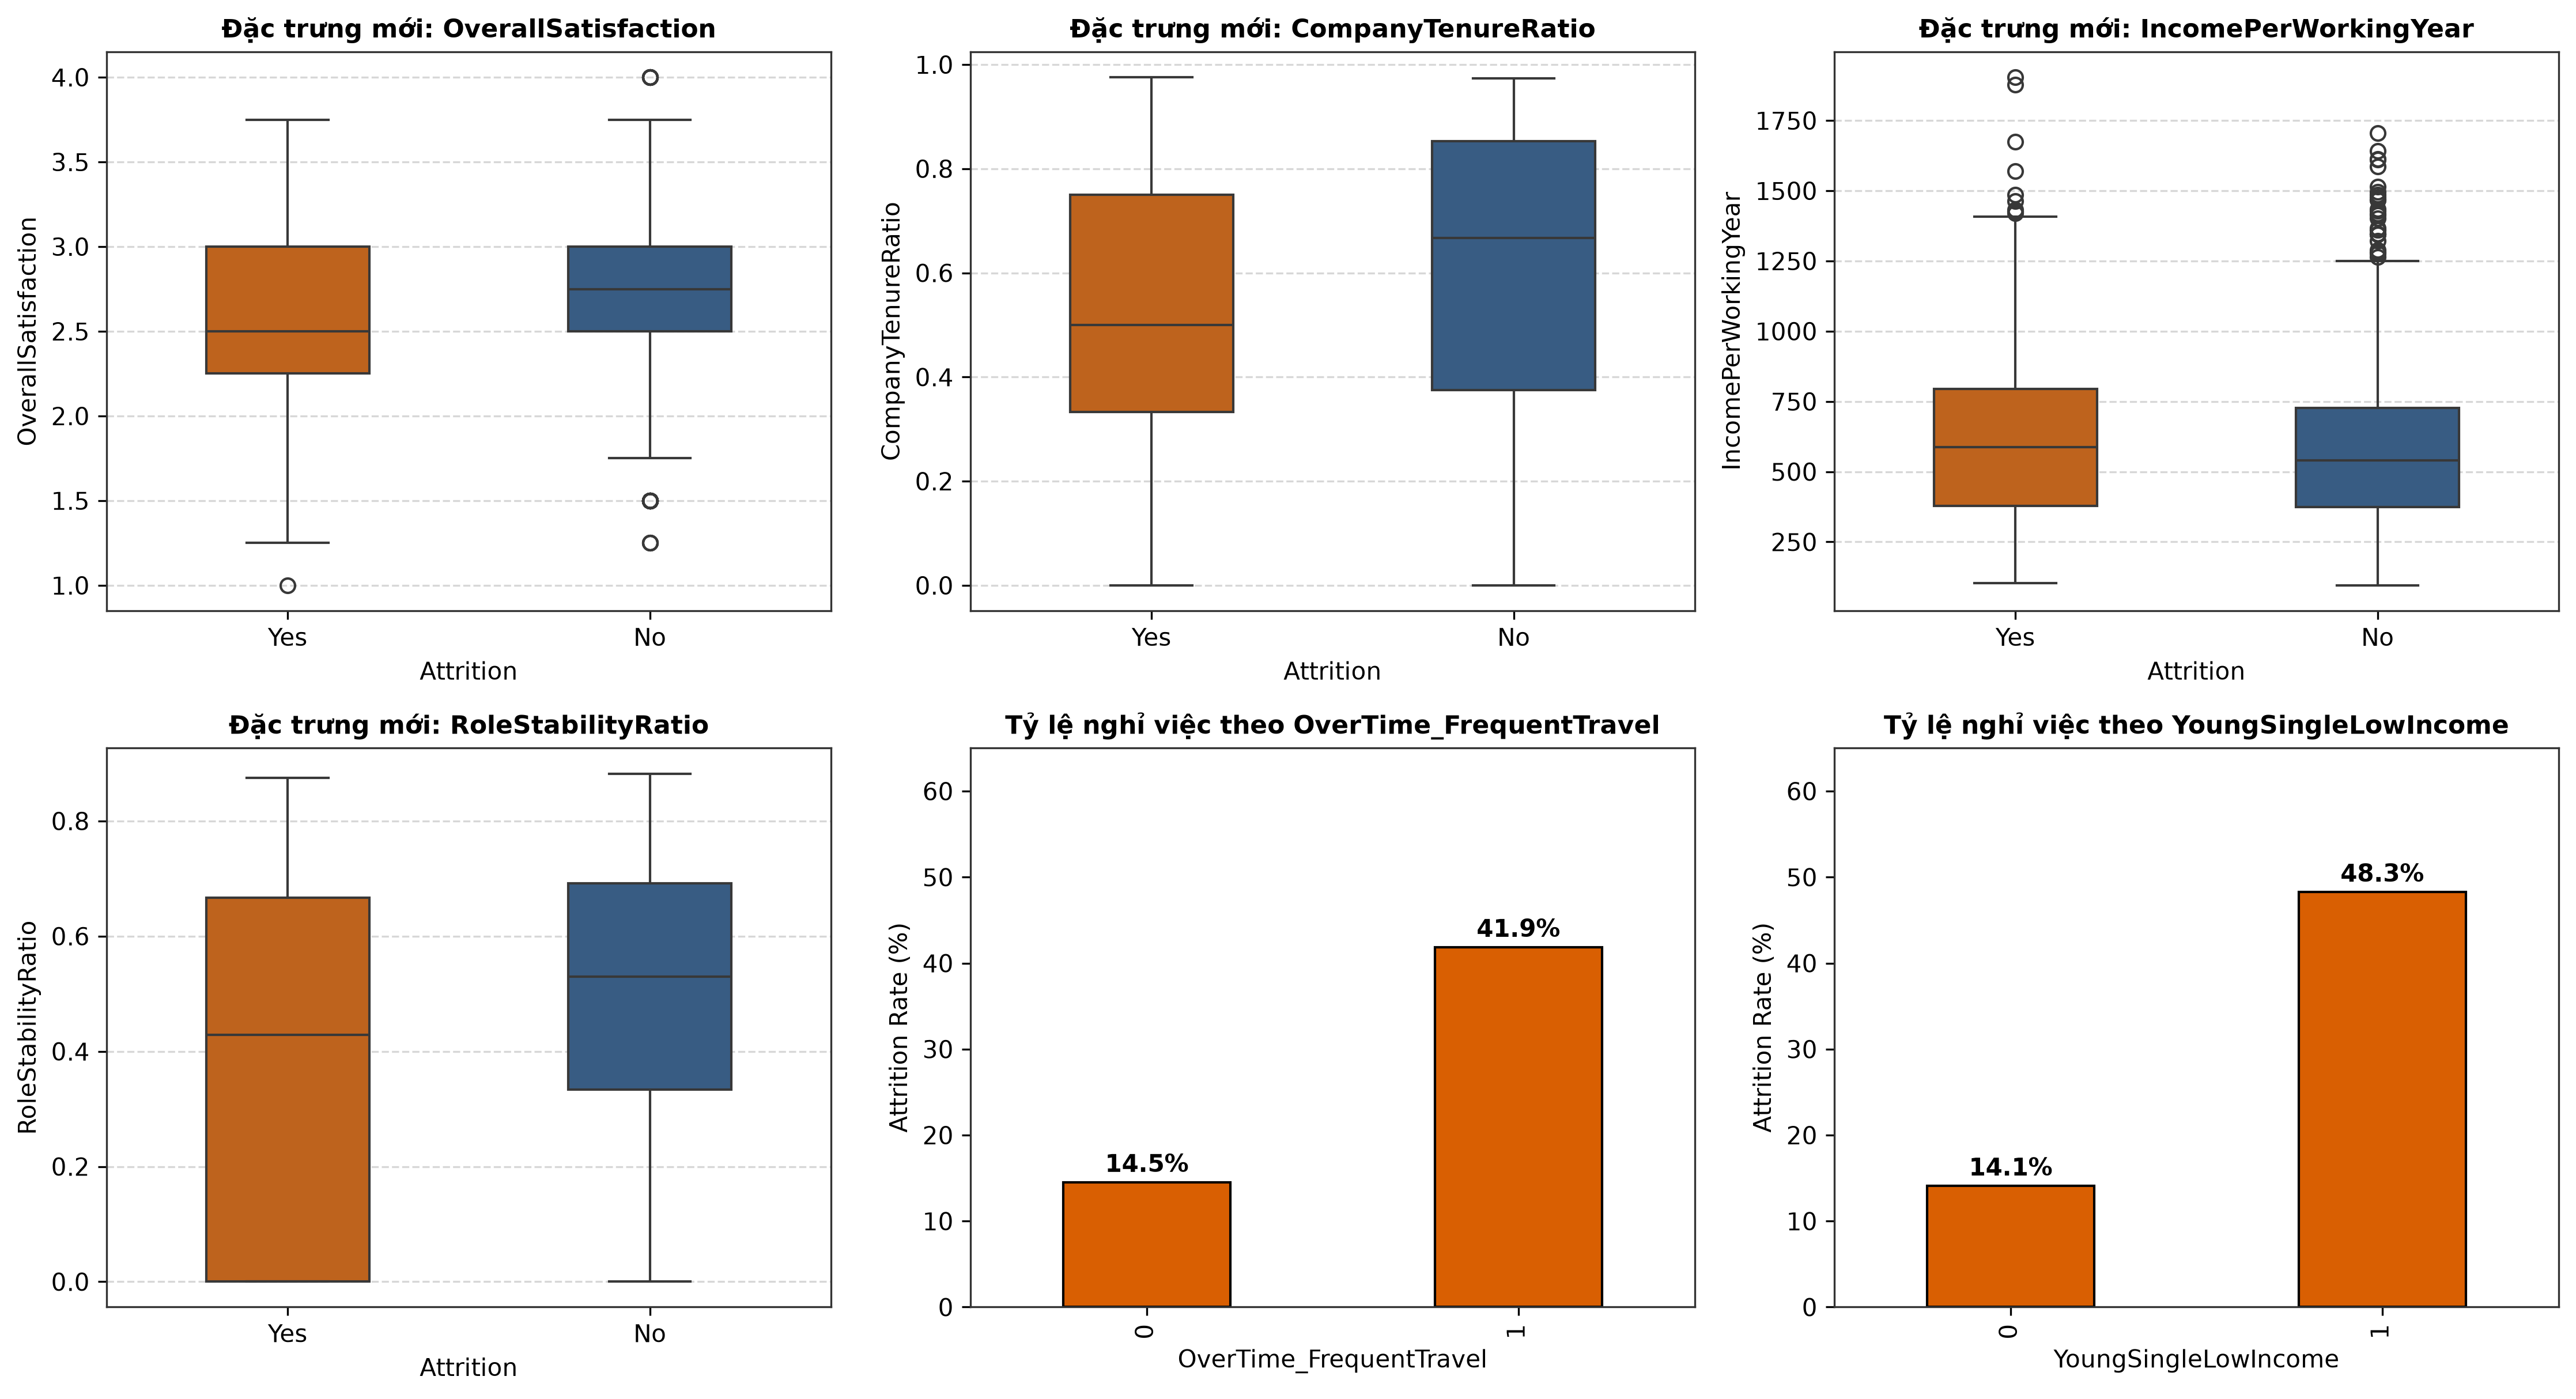
\includegraphics[width=\textwidth]{figures/fig11_engineered_features.png}
        \end{column}
    \end{columns}
\end{frame}

% Slide 5
\begin{frame}{4. Kết quả Thực nghiệm Tổng hợp (Tập Test $N=294$)}
    \scriptsize
    \centering
    \begin{tabular}{l l l c c c c c}
        \toprule
        \textbf{Mô hình} & \textbf{Luồng} & \textbf{Giai đoạn} & \textbf{CV F1} & \textbf{Accuracy} & \textbf{Precision} & \textbf{Recall (Yes)} & \textbf{Test F1} \\
        \midrule
        Dummy (Most Frequent) & Luồng A & Baseline & 0.0000 & 0.8401 & 0.0000 & 0.0000 & 0.0000 \\
        K-NN & Luồng A & Default & 0.2264 & 0.8367 & 0.4545 & 0.1064 & 0.1724 \\
        Gaussian NB & Luồng A & Default & 0.3902 & 0.6156 & 0.2500 & 0.7021 & 0.3687 \\
        Decision Tree & Luồng A & Default & 0.3714 & 0.7585 & 0.2931 & 0.3617 & 0.3238 \\
        \midrule
        K-NN & Luồng A & Tuned & 0.3719 & 0.8469 & 0.5625 & 0.1915 & 0.2857 \\
        Gaussian NB & Luồng A & Tuned & 0.5029 & 0.7891 & 0.3729 & 0.4681 & 0.4151 \\
        Decision Tree & Luồng A & Tuned & 0.4438 & 0.7449 & 0.3409 & 0.6383 & 0.4444 \\
        \midrule
        \textbf{K-NN} & \textbf{Luồng B} & \textbf{Tuned} & 0.3498 & 0.8333 & 0.4615 & 0.2553 & \textbf{0.3288} \\
        \textbf{Gaussian NB} & \textbf{Luồng B} & \textbf{Tuned} & 0.5012 & 0.8027 & 0.4154 & 0.5745 & \textbf{0.4821} \\
        \textbf{Decision Tree} & \textbf{Luồng B} & \textbf{Tuned} & 0.4457 & 0.7279 & 0.3299 & \textbf{0.6809} & \textbf{0.4444} \\
        \textbf{Random Forest (Mở rộng)} & \textbf{Luồng B} & \textbf{Tuned} & \textbf{0.5056} & \textbf{0.8129} & \textbf{0.4394} & 0.6170 & \textbf{0.5133} \\
        \bottomrule
    \end{tabular}
    \vspace{0.2cm}
    \begin{itemize}
        \item \textbf{Luồng B vượt trội Luồng A} trên tất cả các mô hình: Gaussian NB đạt $F_1 = 0.4821$ ($\text{AUC}=0.7507$), Decision Tree đạt $\text{Recall} = 68.09\%$, Random Forest mở rộng đạt $F_1 = 0.5133$ ($\text{AUC}=0.7785$).
    \end{itemize}
\end{frame}

% Slide 6
\begin{frame}{5. So sánh Mô hình, Ma trận nhầm lẫn \& Đường cong ROC}
    \begin{columns}
        \begin{column}{0.55\textwidth}
            \centering
            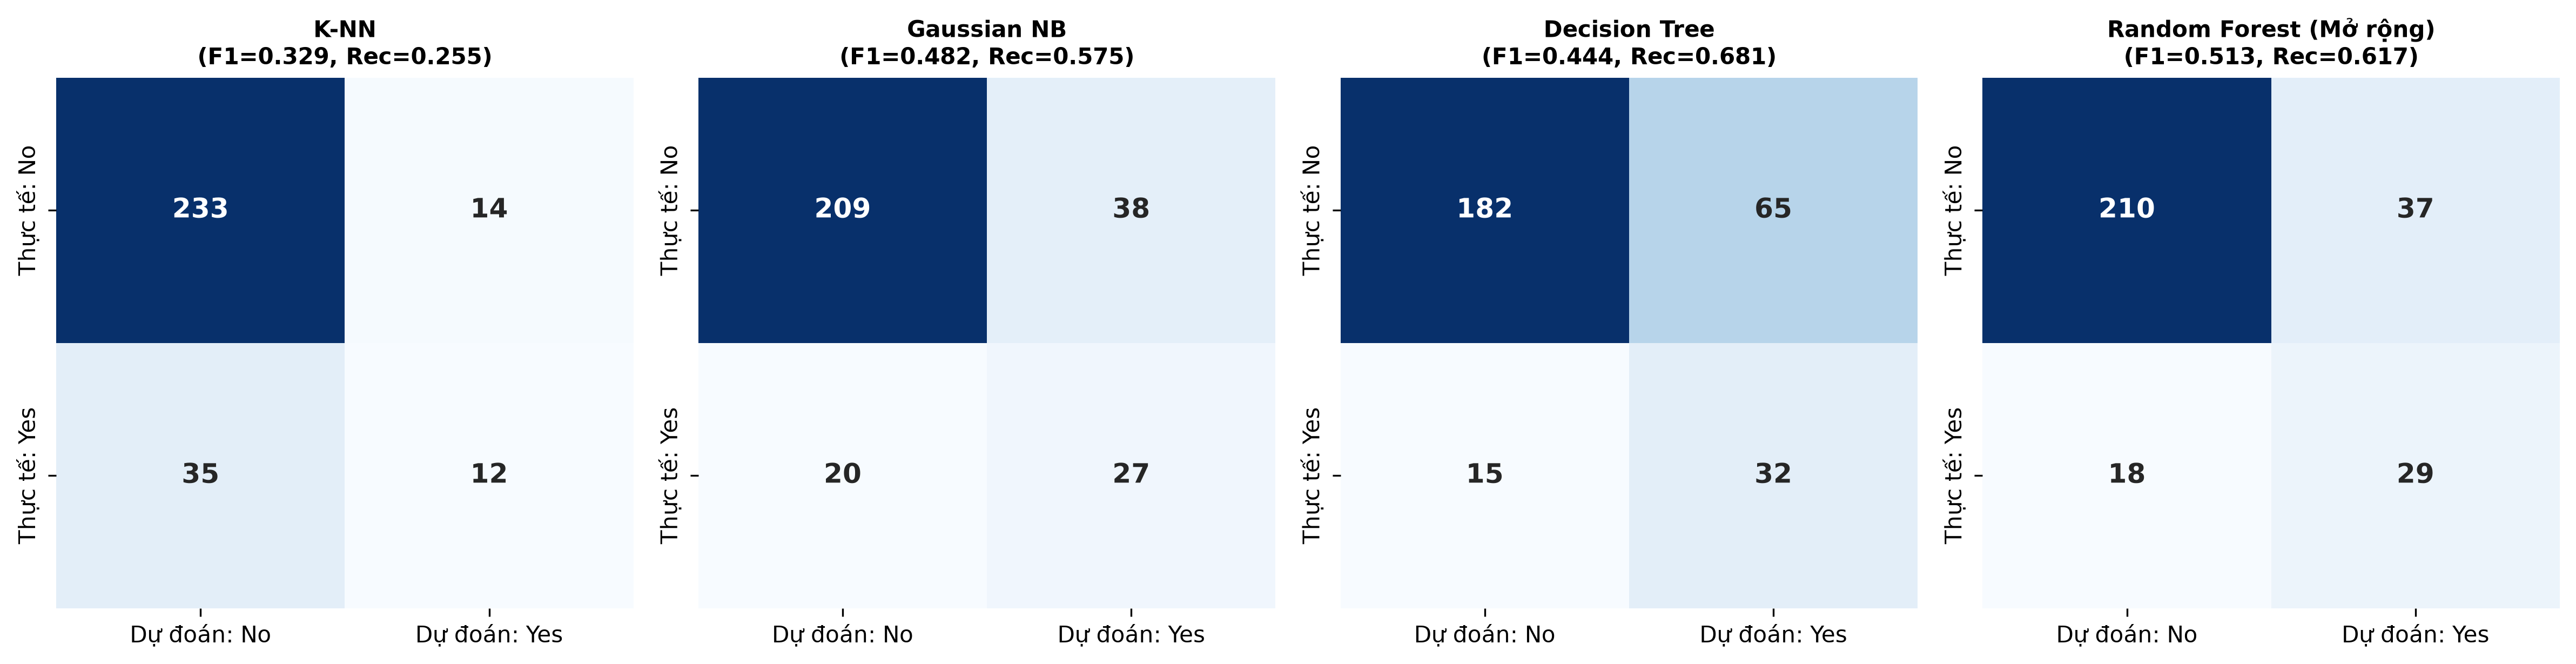
\includegraphics[width=\textwidth]{figures/fig7_confusion_matrices.png}\\[0.2cm]
            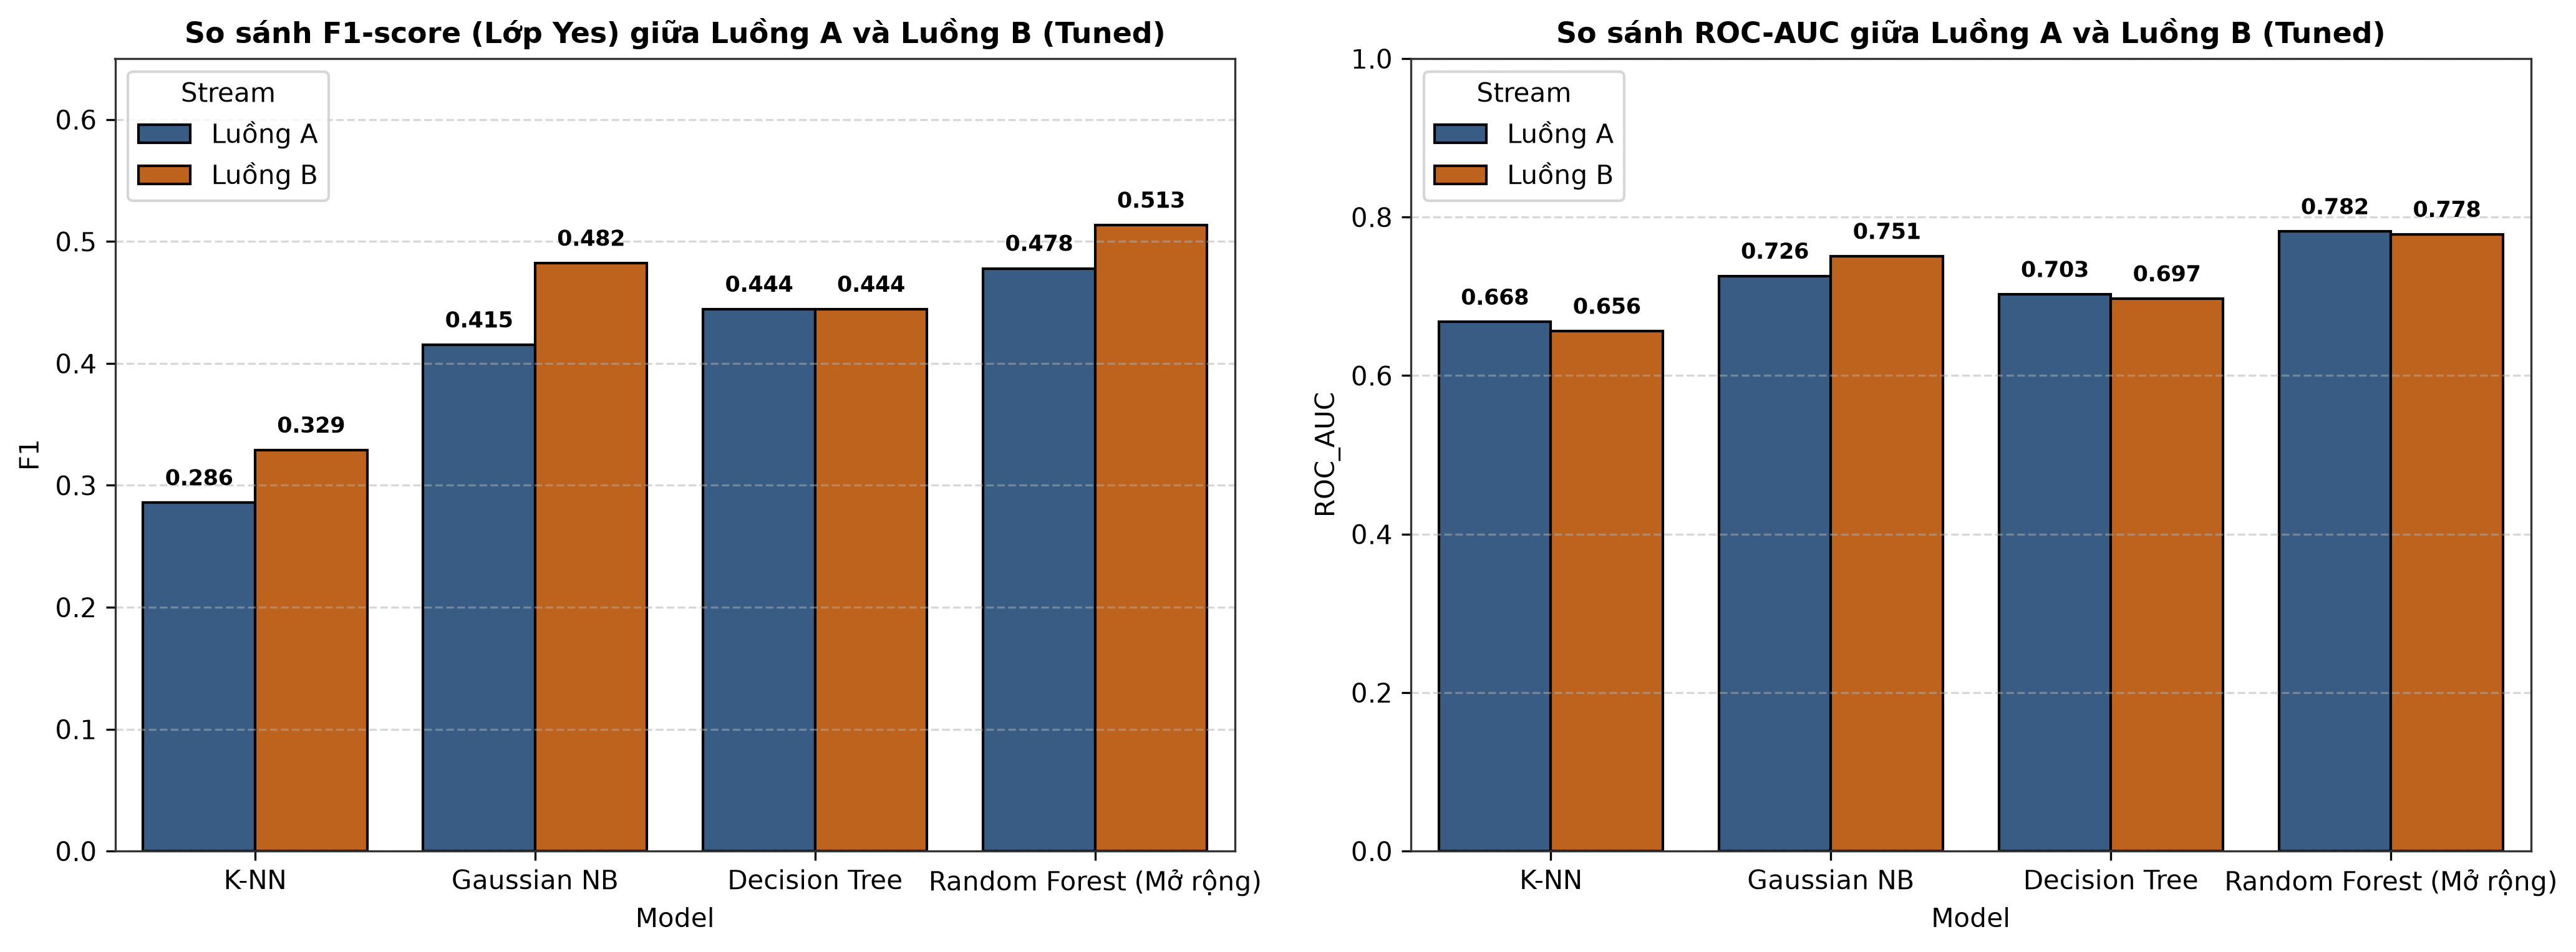
\includegraphics[width=0.92\textwidth]{figures/fig6_model_comparison.png}
        \end{column}
        \begin{column}{0.44\textwidth}
            \centering
            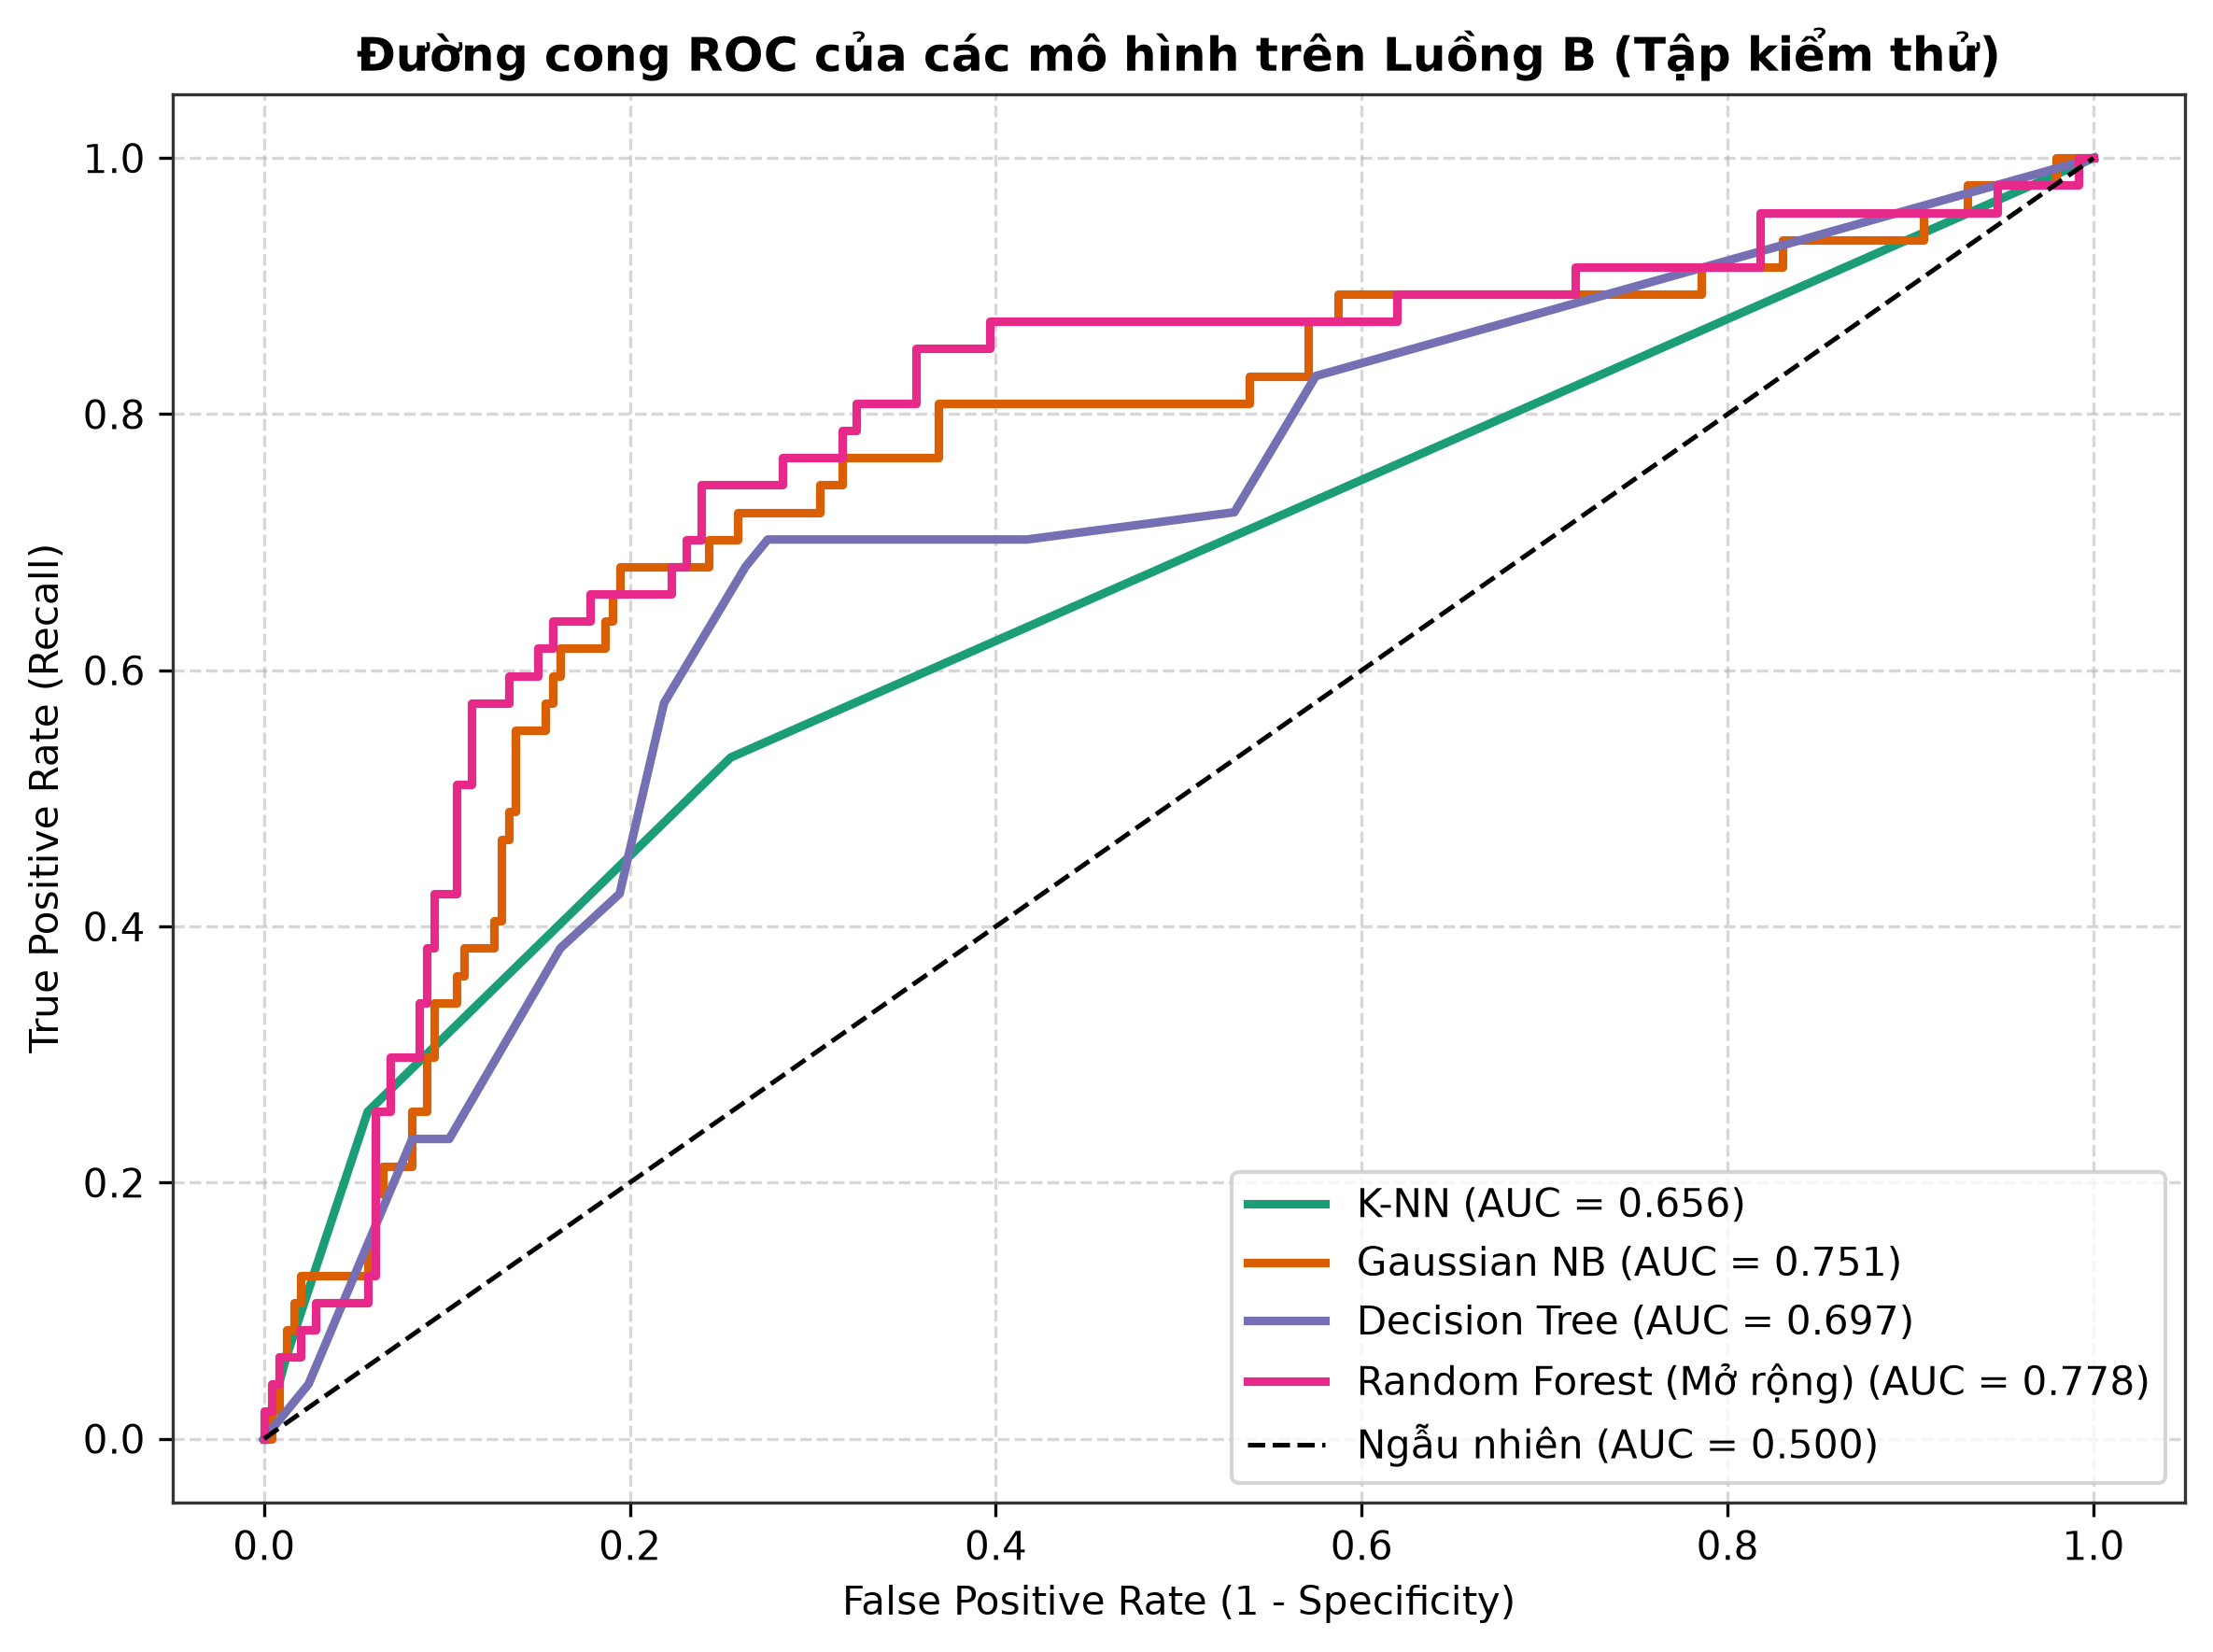
\includegraphics[width=\textwidth]{figures/fig8_roc_curves.png}
        \end{column}
    \end{columns}
\end{frame}

% Slide 7
\begin{frame}{6. Phân tích lỗi (Error Analysis) \& Khuyến nghị Nhân sự}
    \begin{columns}
        \begin{column}{0.52\textwidth}
            \textbf{Mổ xẻ các ca dự đoán sai trên tập Test:}
            \begin{itemize}
                \item \textbf{False Negatives (15 ca bỏ sót):} Điển hình là NV \texttt{\#58} (Lương $\$19{,}545$, không OverTime) và NV \texttt{\#165} (Lương $\$10{,}312$, 40 năm làm việc) nhưng \texttt{YearsSinceLastPromotion = 15 năm} $\rightarrow$ Nghỉ việc do bão hòa sự nghiệp hoặc nghỉ hưu sớm.
                \item \textbf{False Positives (65 ca báo động giả):} Điển hình NV \texttt{\#1495} (24 tuổi, lương $\$2{,}033$, JobSat=2) và NV \texttt{\#434} (27 tuổi, OverTime=Yes) $\rightarrow$ Thực chất là \textbf{nhóm nhân viên có nguy cơ tiềm ẩn cao} cần HR chăm sóc sớm.
            \end{itemize}
        \end{column}
        \begin{column}{0.46\textwidth}
            \centering
            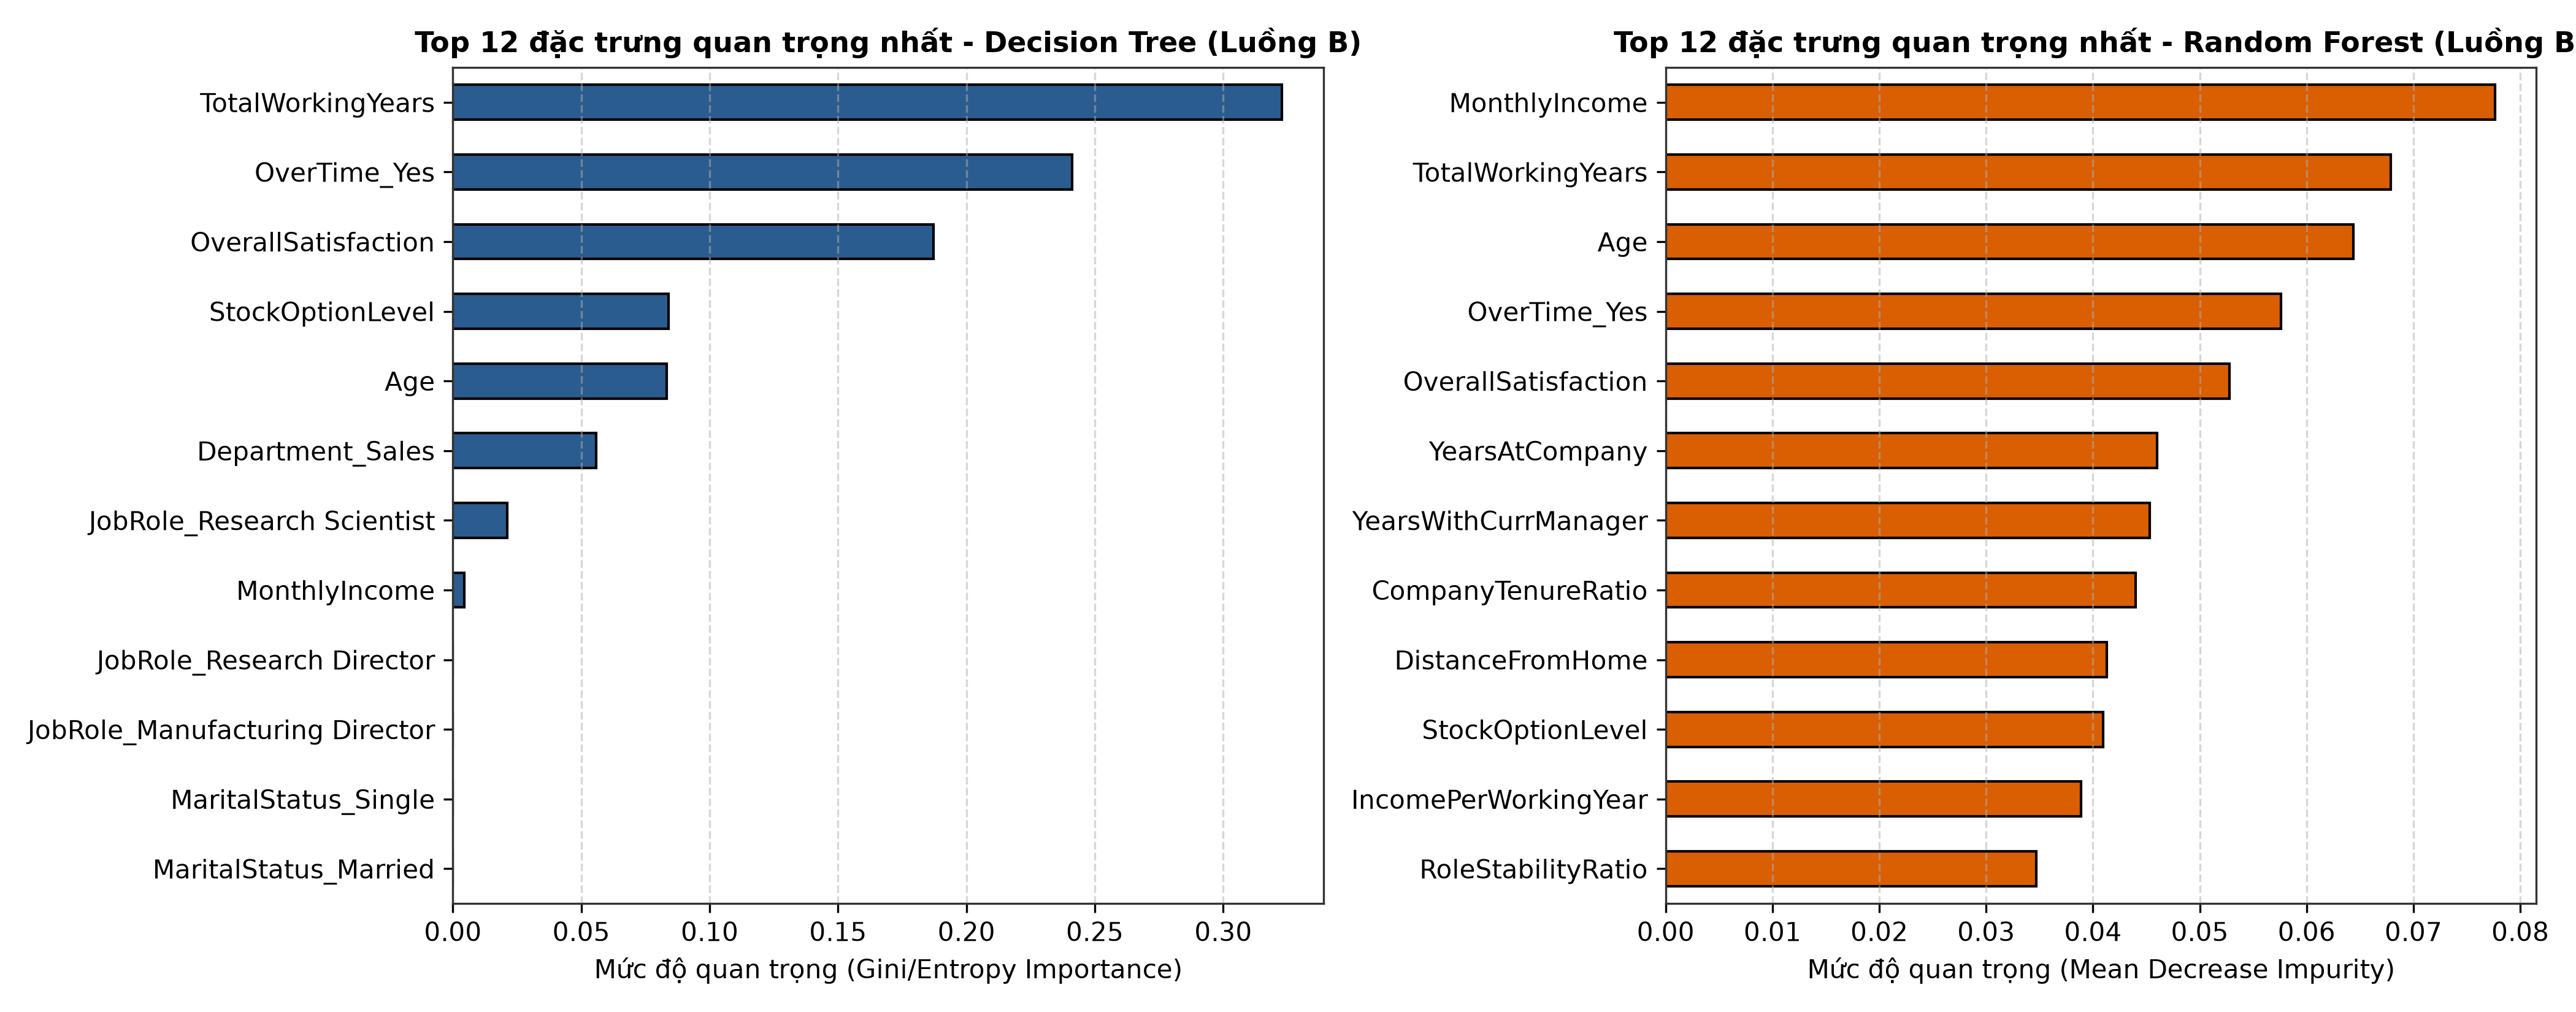
\includegraphics[width=\textwidth]{figures/fig9_feature_importance_tree.png}
            \footnotesize \textbf{Top yếu tố quyết định:} \texttt{OverTime}, \texttt{TotalWorkingYears}, \texttt{MonthlyIncome}, \texttt{OverallSatisfaction}, \texttt{Age}.
        \end{column}
    \end{columns}
\end{frame}

\end{document}
